\begin{figure}[t]
    \centering
    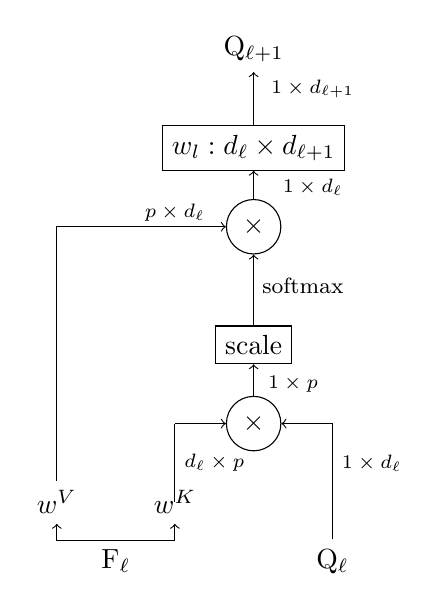
\begin{tikzpicture}
        \node (Q) at (4.5, -1.25) {Q$_\ell$};
        \node (dimq) at (5, 0) {\scriptsize${1\times d_\ell}$};
        \node (wv) at (1, -0.5) {$w^V$};
        \node (wk) at (2.5 , -0.5) {$w^K$};
        \node (F) at (1.75, -1.25) {F$_{\ell}$};
        \node (dimft) at (3.0, -0) {\scriptsize${d_{\ell}\times p}$};
        \node (empt1) at (2.5, 0.5) {};
        \node[shape=circle,draw=black] (mm1) at (3.5, 0.5) {$\times$};
        \node (dimraw) at (4,1) {\scriptsize$1\times p$};
        \node[shape=rectangle,draw=black](scale) at (3.5, 1.5) {scale};
        \node (dimf) at (2.5, 3.175) {\scriptsize${p\times d_{\ell}}$};
        \node (soft) at (4.125, 2.25) {\footnotesize softmax};
        \node[shape=circle,draw=black] (mm2) at (3.5, 3) {$\times$};
        \node[shape=rectangle,draw=black](project) at (3.5, 4) {$w_l: d_\ell\times d_{\ell+1}$ };
        \node (dimscaled) [] at (4.25, 3.5) {\scriptsize $1\times d_\ell$};
        % \node [shape=circle,draw=black](sum1) at (3.5, 4) {+};
        % \node [shape=rectangle,draw=black](norm) at (3.5, 5.75) {LayerNorm};
        \node (Qplus1) at (3.5, 5.25) {Q$_{\ell+1}$};
        \node (dimql) [align=left] at (4.25, 4.75) {\scriptsize$1\times d_{\ell+1}$};
        % \node (empt2) at (5.75, -0.5) {};
        
        \draw[->] (Q) |- node {} (mm1);
        \draw[->] (mm1) -- node {} (scale);
        \draw[->] (scale) -- node {} (mm2);
        \draw[->] (F.north) -| node {} (wv);
        \draw[->] (F.north) -| node {} (wk);
        \draw[-] (wk) -| node {} (empt1.center);
        \draw[->] (empt1.center) |- node {} (mm1);
        \draw[->] (wv.north) |- node {} (mm2);
        
        \draw[->] (mm2) -- node {} (project);
        \draw[->] (project) -- node {} (Qplus1);

    \end{tikzpicture}
    \caption{A Cross Attention Block. We denote matrix multiplication as "$\otimes$". The softmax operation is performed on each row). For a given layer $\ell$ we update our [CLS] token $Q_\ell$; by computing its scaled cross attention with the feature maps $F_\ell$, that are then projected to the channel dimension in the following stage, using a dense layer parametrized by $w_\ell$.}
    \label{fig:fig_crossatt}
\end{figure}